% Slide 16: Linear Regression
\begin{frame}{رگرسیون خطی}{\lr{Linear Regression}}
  \begin{columns}[T]
    \begin{column}{0.56\textwidth}
      \begin{itemize}
        \setlength{\itemsep}{6pt}
        \item \textbf{چگونه تابع رگرسیون خطی را یاد بگیریم؟}
        \item \textbf{فرض اساسی:} متغیر هدف $y$ وابستگی (تقریباً) خطی به متغیرهای توصیفی $X$ دارد.
        \item \textbf{برای تجسم دوبعدی} (یک متغیر مستقل $x$ در رگرسیون ساده):
        \par\vspace{2pt}\noindent\makebox[\linewidth][c]{$f(x) = w_0 + w_1 x$}\par\vspace{2pt}
        \item \textbf{در واقعیت:} بردار ویژگی‌های چندگانه $X = (x_1, \dots, x_n)$ (رگرسیون خطی چندمتغیره).
      \end{itemize}
    \end{column}
    \begin{column}{0.42\textwidth}
      \begin{center}
        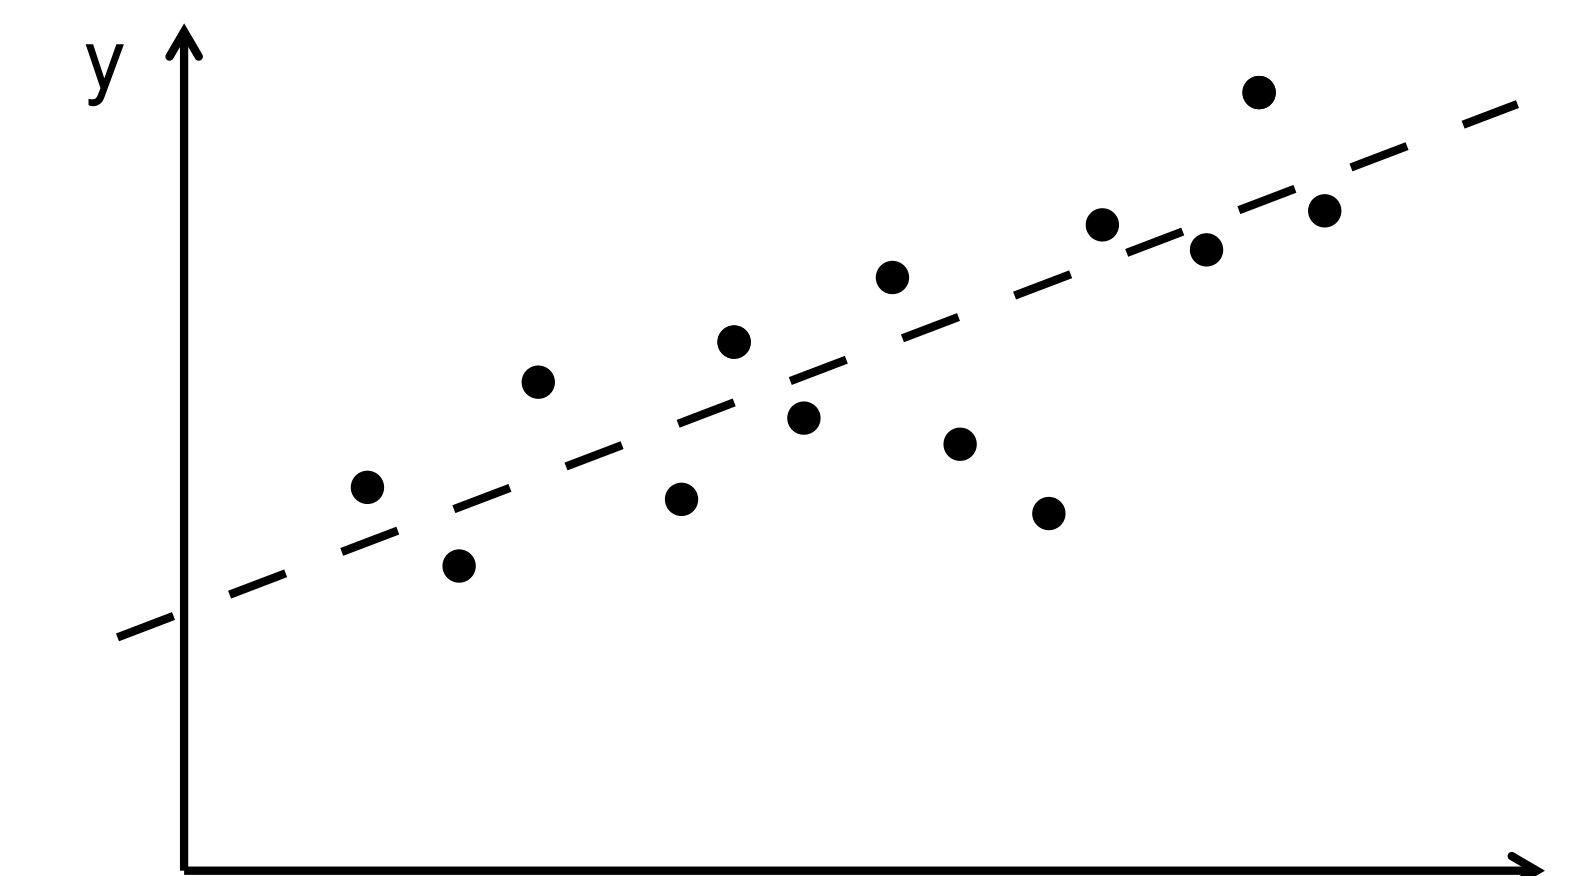
\includegraphics[width=\textwidth,height=4.2cm,keepaspectratio]{images/slide16_linear_fit.png}
      \end{center}
    \end{column}
  \end{columns}
\end{frame}

% Slide 17: Fitting via Least Squares (Simple)
\begin{frame}{برازش تابع رگرسیون: روش کمترین مربعات}{\lr{Least-Squares Approach: Simple Linear Regression}}
  \begin{columns}[T]
    \begin{column}{0.56\textwidth}
      \begin{itemize}
        \setlength{\itemsep}{5pt}
        \item هدف یافتن بردار وزن‌های $W = (w_0, w_1)$ برای تابع $f(x) = w_0 + w_1 x$ است که مجموع مربعات خطا را کمینه کند:
        \par\vspace{2pt}\noindent\makebox[\linewidth][c]{$\displaystyle \text{SSE} = \sum_{i=1}^n (y_i - f(x_i))^2$}\par\vspace{2pt}
        \item \textbf{باقیمانده‌ها} (\lr{Residuals})؛ اختلاف میان مقدار تخمین‌زده‌شده توسط مدل و مقدار واقعی داده آموزش:
        \par\vspace{2pt}\noindent\makebox[\linewidth][c]{$e_i = y_i - f(x_i)$}\par\vspace{2pt}
      \end{itemize}
    \end{column}
    \begin{column}{0.42\textwidth}
      \begin{center}
        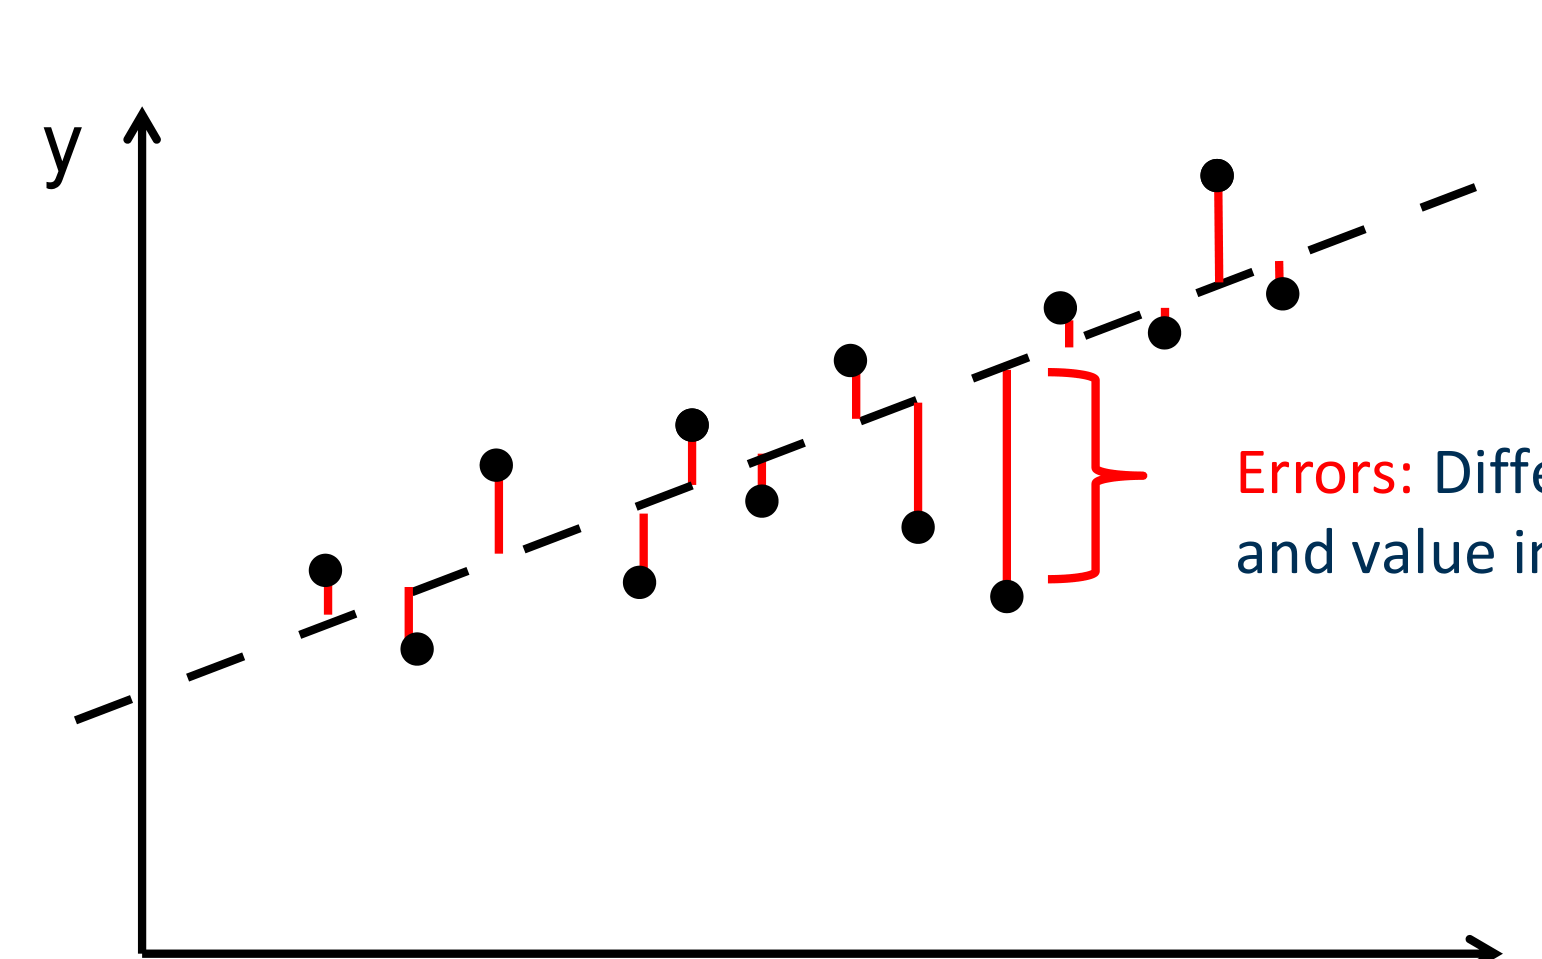
\includegraphics[width=\textwidth,height=4.2cm,keepaspectratio]{images/slide17_least_squares_residuals.png}
      \end{center}
    \end{column}
  \end{columns}
\end{frame}

% Slide 18: Multiple Linear Regression
\begin{frame}{رگرسیون خطی چندمتغیره}{\lr{Multiple Linear Regression}}
  \begin{columns}[T]
    \begin{column}{0.64\textwidth}
      \begin{itemize}
        \setlength{\itemsep}{5pt}
        \item برازش ابرصفحهٔ رگرسیون برای $n$ متغیر توصیفی:
        \par\vspace{2pt}\noindent\makebox[\linewidth][c]{$\displaystyle \hat{y}(X) = w_0 + w_1 x_1 + w_2 x_2 + \dots + w_n x_n$}\par\vspace{2pt}
        \item کمینه‌سازی معیار \lr{SSE} (مجموع مربعات خطا):
        \par\vspace{2pt}\noindent\makebox[\linewidth][c]{$\displaystyle \text{SSE} = \sum_{i=1}^n \left(y_i - \hat{y}(X_i, W)\right)^2$}\par\vspace{2pt}
        \item حل تحلیلی به کمک معادلهٔ نرمال ماتریسی:
        \par\vspace{2pt}\noindent\makebox[\linewidth][c]{$\displaystyle W = (X^T X)^{-1} X^T Y$}\par\vspace{2pt}
      \end{itemize}
    \end{column}
    \begin{column}{0.34\textwidth}
      \begin{center}
        \vspace{0.2cm}
        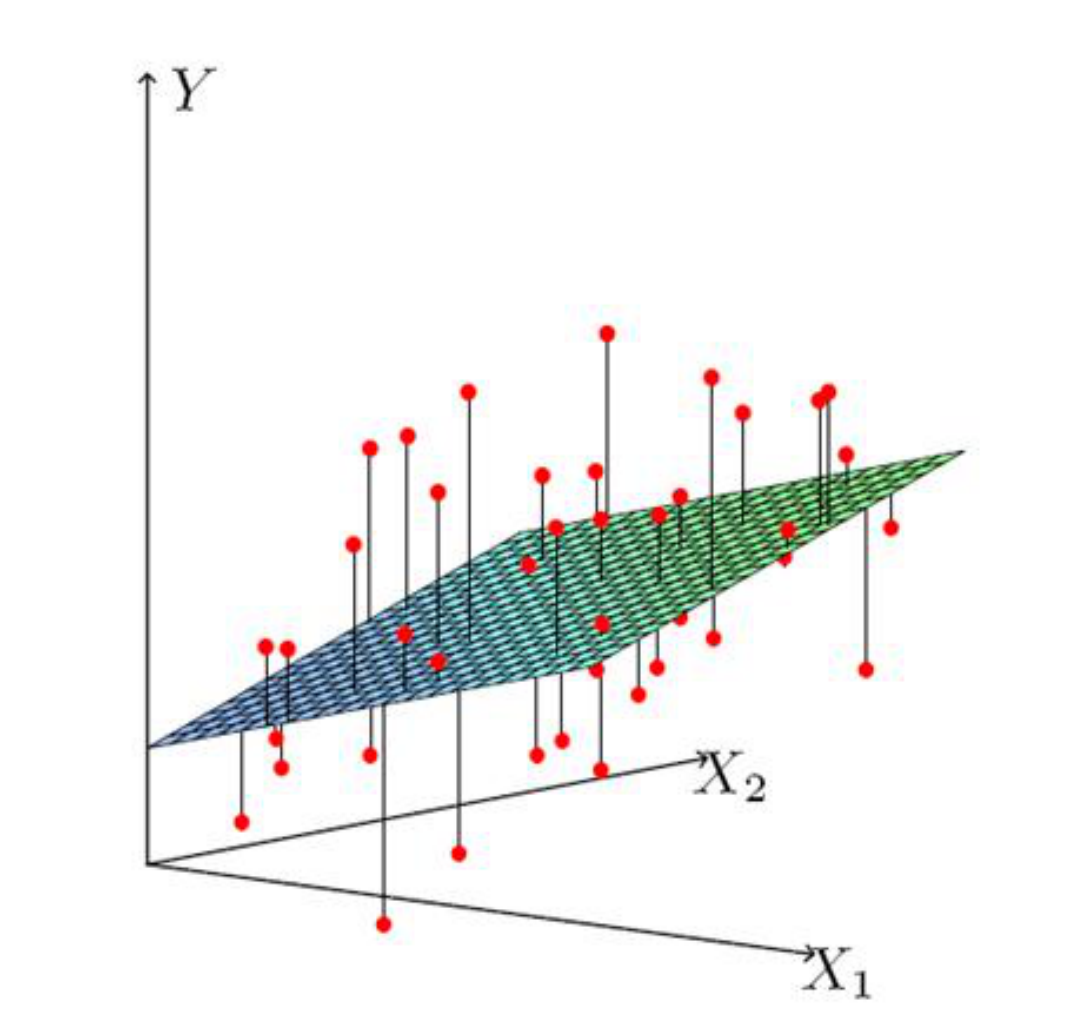
\includegraphics[width=\textwidth,height=4.2cm,keepaspectratio]{images/slide18_multiple_regression_3d.png}
      \end{center}
    \end{column}
  \end{columns}
\end{frame}

% Slide 19: Linear Regression & Overfitting
\begin{frame}{رگرسیون خطی و بیش‌برازش}{\lr{Linear Regression and Overfitting}}
  \begin{columns}[T]
    \begin{column}{0.58\textwidth}
      \begin{itemize}
        \setlength{\itemsep}{6pt}
        \item فرض کنید دو مدل رگرسیونی برای یک پدیده ارائه شده است:
        \begin{itemize}
          \item مدل اول: استفاده از ۵ متغیر برای تبیین پدیده.
          \item مدل دوم: استفاده از ۱۰۰ متغیر برای همان داده‌ها!
        \end{itemize}
        \item کدام مدل ارجح است؟
        \item \textbf{یادآوری تیغ اوکام:} \lr{(Occam's Razor)}
        از میان دو نظریه که پدیده‌ای یکسان را توضیح می‌دهند، همواره مدل ساده‌تر (با متغیرهای کمتر) ترجیح داده می‌شود.
      \end{itemize}
    \end{column}
    \begin{column}{0.40\textwidth}
      \begin{center}
        
\includegraphics[width=\textwidth,height=3.8cm,keepaspectratio]{images/slide19_overfitting_curve.png}
      \end{center}
    \end{column}
  \end{columns}
\end{frame}

% Slide 20: Ridge Regression
\begin{frame}{رگرسیون ریج}{\lr{Ridge Regression ($L_2$ Regularization)}}
  \begin{columns}[T]
    \begin{column}{0.56\textwidth}
      \begin{itemize}
        \setlength{\itemsep}{4pt}
        \item رویکردی بر پایه کمترین مربعات که با کوچک نگه‌داشتن وزن‌ها ($W$) از بیش‌برازش جلوگیری می‌کند.
        \item افزودن جریمه مربعی به وزن‌ها (\lr{Penalty}):
      \end{itemize}
      \vspace{-0.1cm}
      \begin{center}
        {\fontsize{8.5}{11}\selectfont $\displaystyle \min_W \sum_{i=1}^n (y_i - \hat{y}(X_i, W))^2 + \lambda \sum_{j=1}^m w_j^2$}
      \end{center}
      \vspace{-0.1cm}
      \begin{itemize}
        \item \textbf{نقش فراپارامتر $\lambda$ در مدل:}
        \begin{itemize}
          \item به ازای $\lambda=0$: رگرسیون خطی معمولی (\lr{OLS}) بدون جریمه.
          \item برای مقادیر بزرگ $\lambda$: انقباض ضرایب به سمت صفر (\lr{Shrinkage}).
        \end{itemize}
      \end{itemize}
    \end{column}
    \begin{column}{0.42\textwidth}
      \begin{center}
        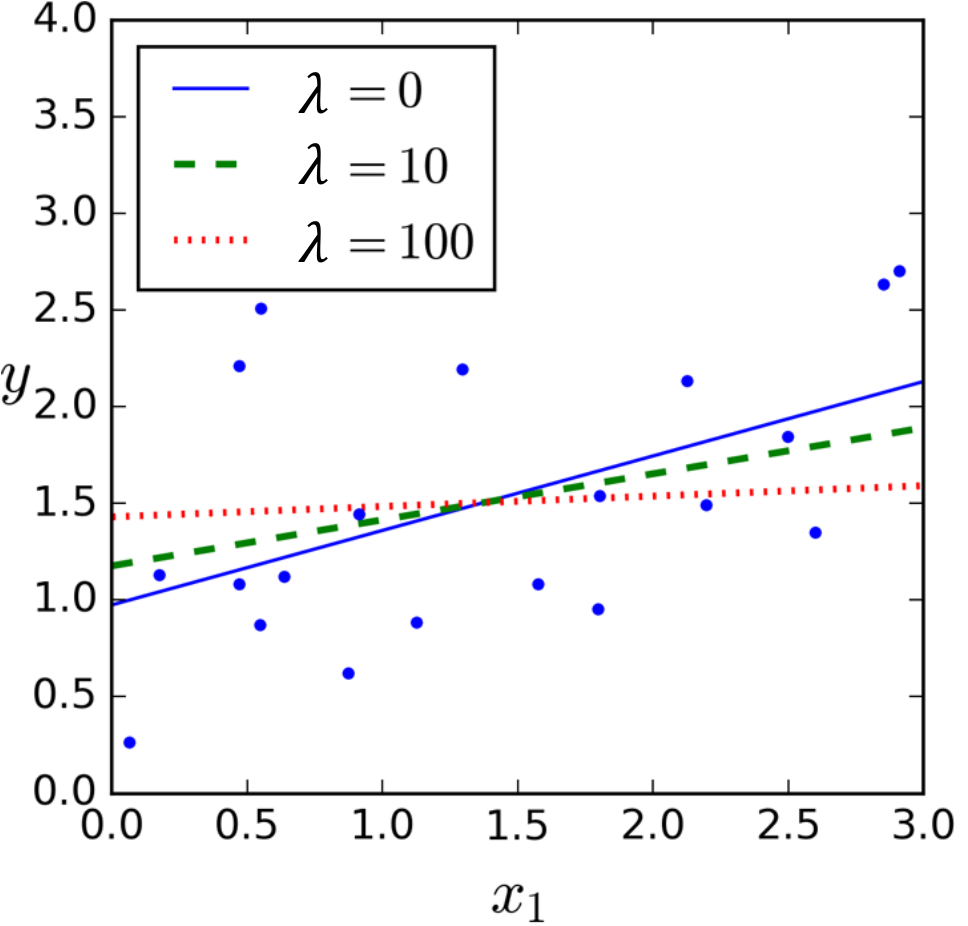
\includegraphics[width=\textwidth,height=4.2cm,keepaspectratio]{images/slide20_ridge_shrinkage.png}
      \end{center}
    \end{column}
  \end{columns}
\end{frame}

% Slide 21: Lasso Regression
\begin{frame}{رگرسیون لاسو}{\lr{Lasso Regression ($L_1$ Regularization)}}
  \begin{itemize}
    \setlength{\itemsep}{4pt}
    \item رگرسیون ریج ضرایب را کوچک می‌کند اما دقیقاً صفر نمی‌سازد.
    \item \textbf{رگرسیون لاسو:} ضرایب ویژگی‌های غیرضروری را دقیقاً به \textbf{صفر} کاهش می‌دهد (انتخاب ویژگی توکار).
    \item تابع هدف بهینه‌سازی لاسو با جریمه قدرمطلق:
    \par\vspace{2pt}\noindent\makebox[\linewidth][c]{$\displaystyle \min_W \sum_{i=1}^n (y_i - \hat{y}(X_i, W))^2 + \lambda \sum_{j=1}^m |w_j|$}\par\vspace{2pt}
    \item \textbf{رفتار حدی فراپارامتر $\lambda$ در مدل:}
    \begin{itemize}
      \item به ازای $\lambda = 0$: بدون منظم‌سازی (رگرسیون خطی معمولی) $\rightarrow$ خطر بیش‌برازش (\lr{Overfitting}).
      \item وقتی $\lambda \to \infty$: میل تمام وزن‌ها به سمت صفر $\rightarrow$ کم‌برازش شدید (\lr{Underfitting}).
    \end{itemize}
  \end{itemize}
\end{frame}

% Slide 22: Lasso vs. Ridge Regression
\begin{frame}{مقایسه هندسی لاسو و ریج}{\lr{Lasso vs. Ridge Regression: Geometry}}
  \begin{itemize}
    \setlength{\itemsep}{3pt}
    \item در لاسو، برای مقادیر $|w_i|$ نزدیک به صفر، شیب جریمه خطی بزرگتر از جریمه مربعی ریج باقی می‌ماند.
    \item به همین دلیل، فرآیند بهینه‌سازی وزن‌های کم‌اهمیت را دقیقاً روی محورها بر صفر منطبق می‌سازد (\lr{Sparsity}).
  \end{itemize}
  \begin{center}
    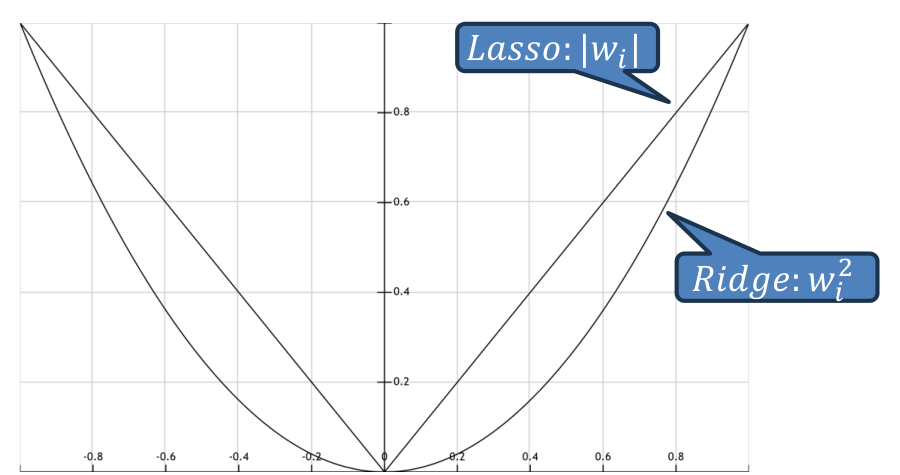
\includegraphics[width=0.88\textwidth,height=3.6cm,keepaspectratio]{images/slide22_lasso_vs_ridge_geometry.png}\\[0.1cm]
    {\fontsize{8}{10}\selectfont\color{subgray}مقایسه هندسی: لوزی (مدل \lr{Lasso} با جریمه خطی) در برابر دایره (مدل \lr{Ridge} با جریمه مربعی)}
  \end{center}
\end{frame}

% Slide 23: Interpolation vs. Extrapolation
\begin{frame}{درون‌یابی در برابر برون‌یابی}{\lr{Interpolation vs. Extrapolation}}
  \begin{columns}[T]
    \begin{column}{0.54\textwidth}
      \begin{itemize}
        \setlength{\itemsep}{5pt}
        \item \textbf{داده‌های آموزش:}
        مشاهدات روزانه هواشناسی (دما، سرعت باد، رطوبت) در بازه \lr{$[-15^\circ\mathrm{C}, 32^\circ\mathrm{C}]$}.
        \item \textbf{رگرسیون درون‌یاب} (\lr{Interpolating})
        تنها مقادیری در محدوده بازه آموزشی داده‌ها پیش‌بینی می‌کند.
        \item \textbf{رگرسیون برون‌یاب} (\lr{Extrapolating})
        قادر است مقادیر فراتر یا خارج از بازه دیده‌شده را نیز پیش‌بینی نماید.
      \end{itemize}
    \end{column}
    \begin{column}{0.44\textwidth}
      \begin{center}
        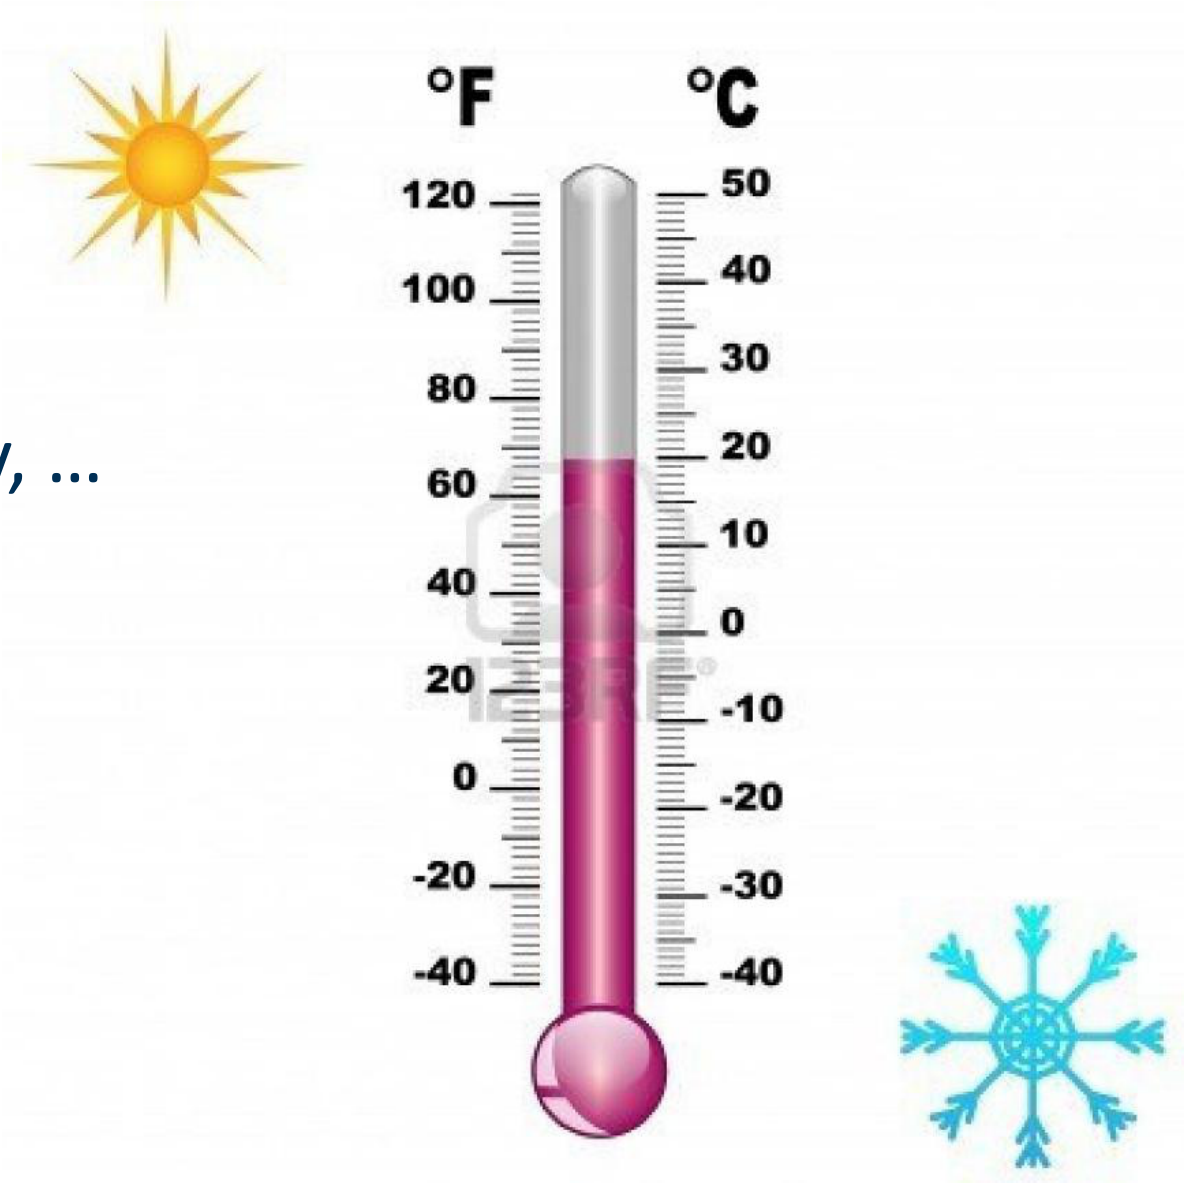
\includegraphics[width=\textwidth,height=3.8cm,keepaspectratio]{images/slide23_extrapolation_warning.png}
      \end{center}
    \end{column}
  \end{columns}
\end{frame}

% Slide 24: Interpolation is Safe
\begin{frame}{درون‌یابی به عنوان رویکردی «امن»}{\lr{Interpolation as a Safe Strategy}}
  \begin{itemize}
    \setlength{\itemsep}{3pt}
    \item رگرسیون‌های درون‌یاب عموماً «امن» تلقی می‌شوند، زیرا فقط مقادیر منطقی و باورپذیر را تخمین می‌زنند.
  \end{itemize}
  \begin{center}
    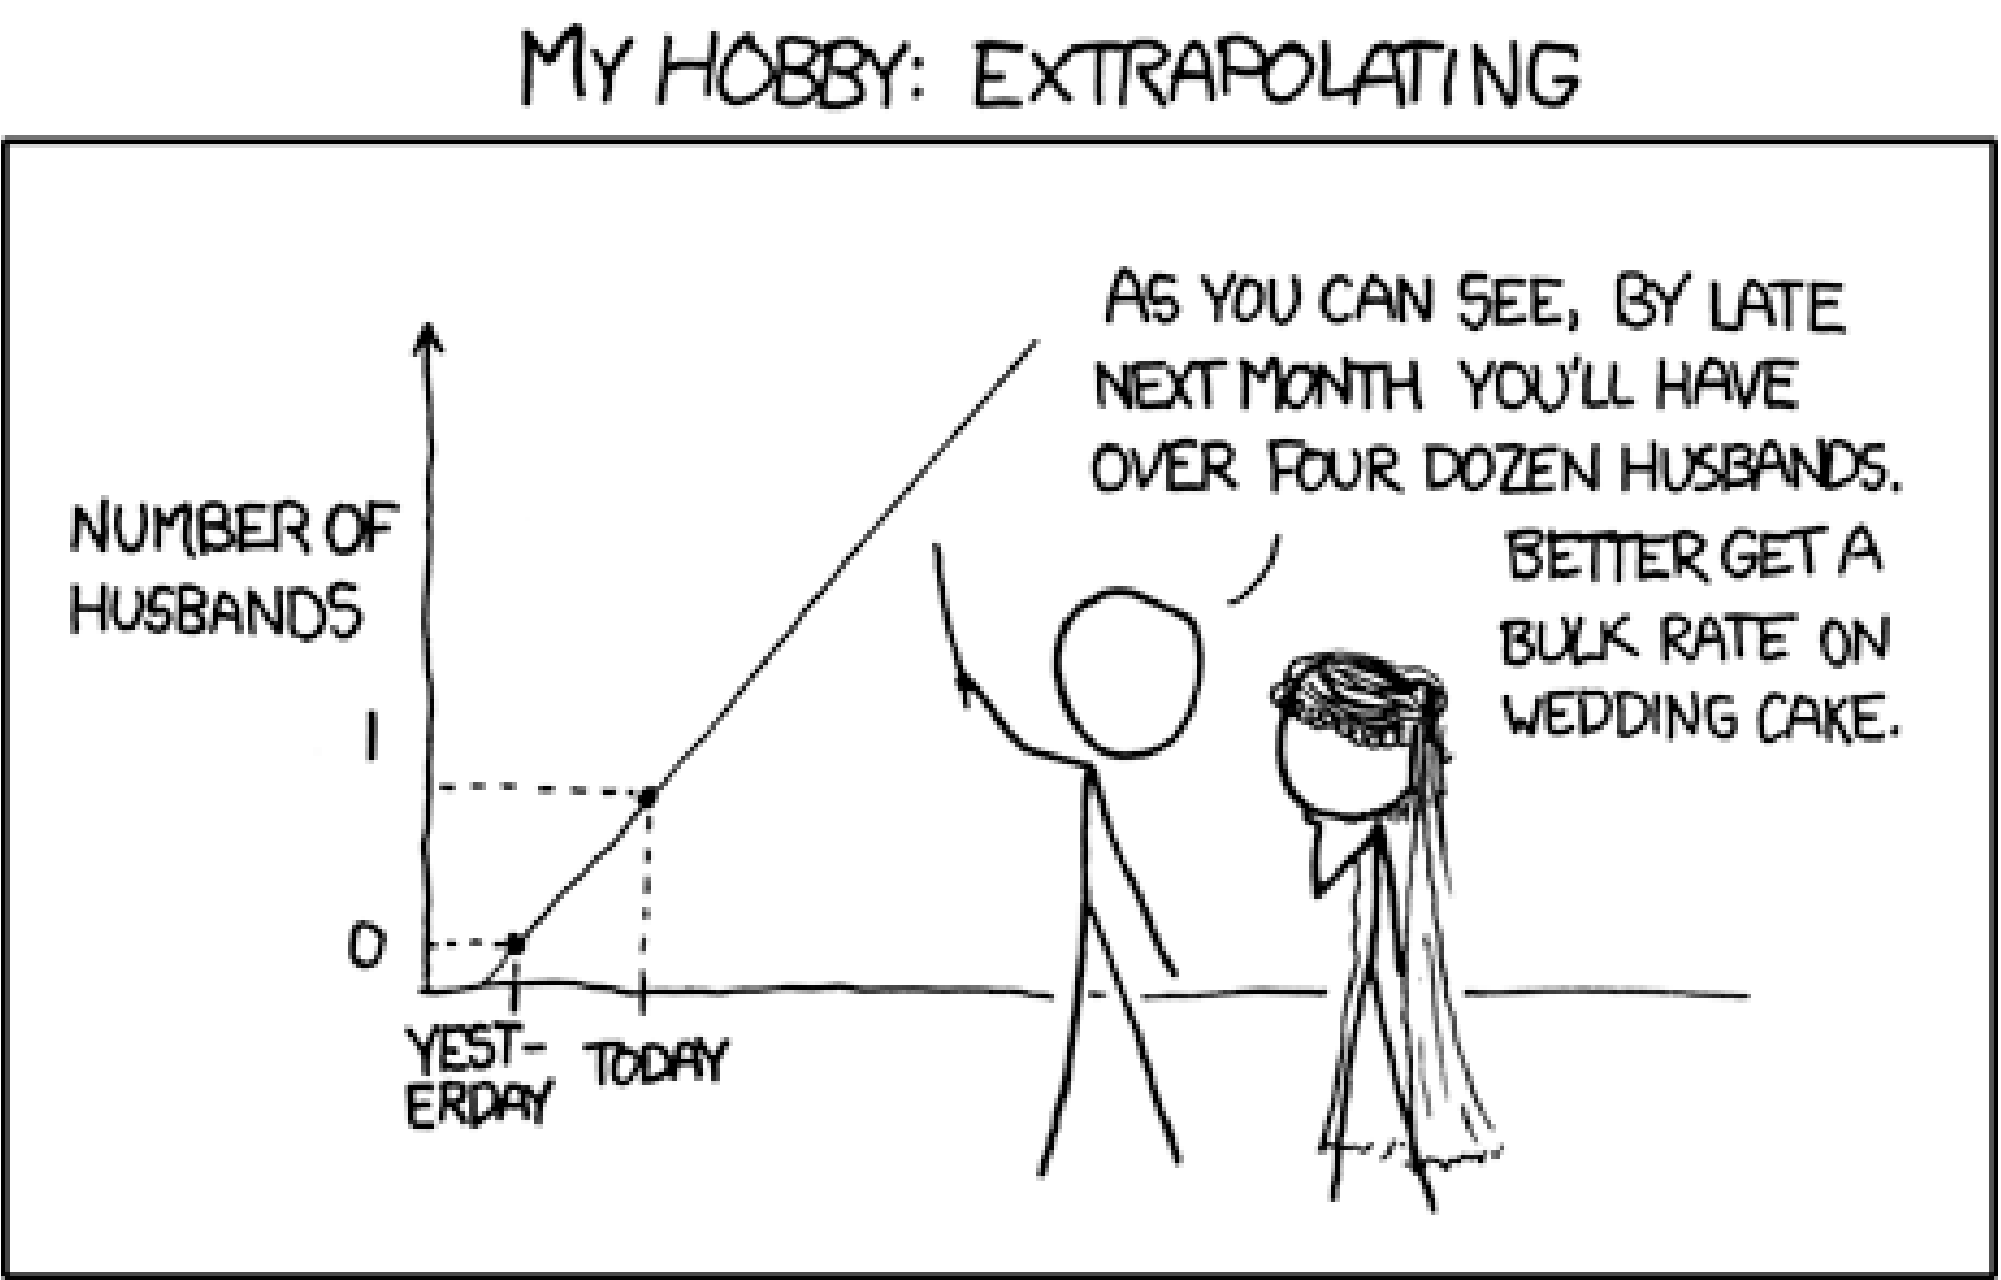
\includegraphics[width=0.72\textwidth,height=4.0cm,keepaspectratio]{images/slide24_xkcd_extrapolation.png}
  \end{center}
\end{frame}

% Slide 25: When Extrapolation is Needed
\begin{frame}{چه زمانی برون‌یابی ضروری است؟}{\lr{When Extrapolation is Needed}}
  \begin{columns}[T]
    \begin{column}{0.52\textwidth}
      \begin{itemize}
        \setlength{\itemsep}{6pt}
        \item گاهی اوقات تنها پیش‌بینی‌های برون‌یابی جذاب و کاربردی هستند:
        \begin{itemize}
          \setlength{\itemsep}{4pt}
          \item سطح آب دریاها تا سال ۲۰۵۰ چقدر افزایش خواهد یافت؟
          \item دمای راکتور در یک سناریوی اضطراری تا چه میزانی بالا می‌رود؟
        \end{itemize}
        \item در این کاربردها، مدل‌های درون‌یاب صرفاً مقادیر گذشته را بازگو کرده و ناتوان خواهند بود.
      \end{itemize}
    \end{column}
    \begin{column}{0.46\textwidth}
      \begin{center}
        
\includegraphics[width=\textwidth,height=3.8cm,keepaspectratio]{images/slide25_sea_level_extrapolation.png}
      \end{center}
    \end{column}
  \end{columns}
\end{frame}

% Slide 26: Linear vs KNN Regression
\begin{frame}{مقایسه رگرسیون خطی و رگرسیون $k$ نزدیک‌ترین همسایه}{\lr{Linear Regression vs. K-NN Regression}}
  \begin{columns}[c]
    \begin{column}{0.45\textwidth}
      \begin{itemize}
        \setlength{\itemsep}{12pt}
        \item \textbf{رگرسیون خطی:}
        \begin{itemize}
          \setlength{\itemsep}{2pt}
          \item برون‌یابی می‌کند
          \item {\small\color{subgray}\lr{Extrapolates}}
        \end{itemize}
        \item \textbf{رگرسیون $k$ نزدیک‌ترین همسایه:}
        \begin{itemize}
          \setlength{\itemsep}{2pt}
          \item درون‌یابی می‌کند
          \item {\small\color{subgray}\lr{Interpolates}}
        \end{itemize}
        \item \textbf{درخت‌های رگرسیون:}
        \begin{itemize}
          \setlength{\itemsep}{2pt}
          \item درون‌یابی می‌کنند
          \item {\small\color{subgray}\lr{Interpolates}}
        \end{itemize}
      \end{itemize}
    \end{column}
    \begin{column}{0.53\textwidth}
      \begin{center}
        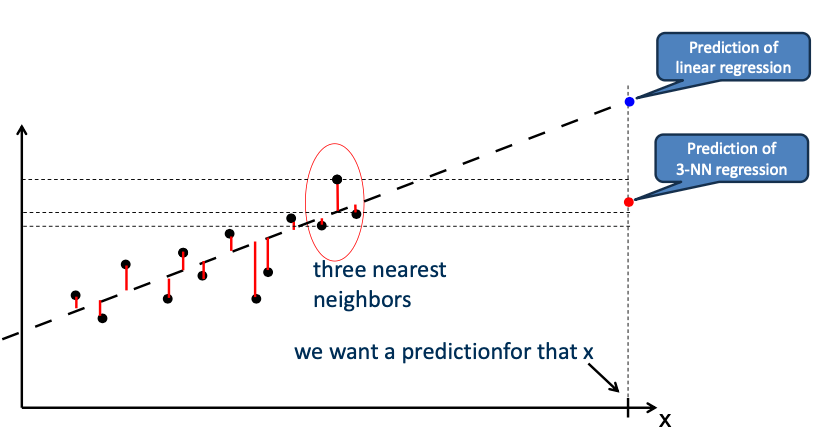
\includegraphics[width=\textwidth,height=5.0cm,keepaspectratio]{images/slide26_linear_vs_knn_clean.png}
      \end{center}
    \end{column}
  \end{columns}
\end{frame}

% Slide 27: Baseline Prediction
\begin{frame}{پیش‌بینی خط پایه در رگرسیون}{\lr{Baseline Prediction}}
  \begin{columns}[T]
    \begin{column}{0.54\textwidth}
      \begin{itemize}
        \setlength{\itemsep}{5pt}
        \item \textbf{در طبقه‌بندی:} پیش‌بینی فراوان‌ترین برچسب (\lr{Majority Class}).
        \item \textbf{در رگرسیون:} پیش‌بینی با مقادیر خلاصه آماری:
        \begin{itemize}
          \item میانگین داده‌ها (\lr{Average / Mean})
          \item میانه داده‌ها (\lr{Median})
          \item مد داده‌ها (\lr{Mode})
        \end{itemize}
        \item در هر صورت: این روش‌ها فقط درون‌یابی انجام می‌دهند.
        \item این مدل‌های ساده خط پایه‌ای قوی برای سنجش ارزش مدل‌های پیچیده هستند.
      \end{itemize}
    \end{column}
    \begin{column}{0.44\textwidth}
      \begin{center}
        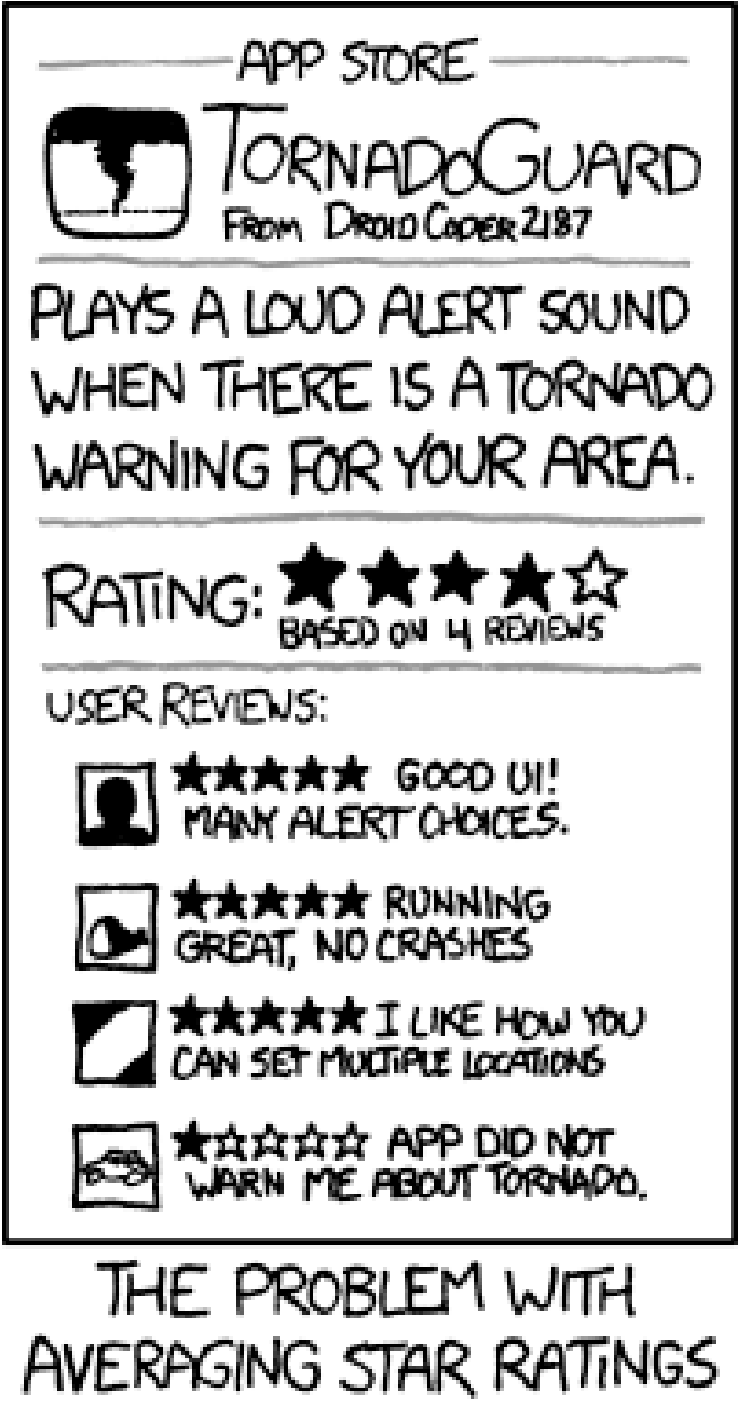
\includegraphics[width=\textwidth,height=4.2cm,keepaspectratio]{images/slide27_xkcd_baseline.png}
      \end{center}
    \end{column}
  \end{columns}
\end{frame}
